\documentclass[12pt]{article}
\usepackage[margin=1in]{geometry}
\usepackage{amsmath}
\usepackage{graphicx}

\title{E155 Final Project Status Report: $\mu$Mudd Mark V Debugging and Lab 6 Revision}
\author{Christopher Ferrarin and Kaveh Pezeshki}
\date{31 November 2018}

\begin{document}
	\begin{LARGE}
	\noindent
		E155 
		Final 
		Project 
		Status
		Report: 
		$\mu$Mudd 
		Mark V \\
		Debugging 
		and 
		Lab 
		6 
		Revision
	\end{LARGE}

	\vspace{0.2cm}
	
	\begin{large}
	Christopher Ferrarin and Kaveh Pezeshki
	
	31 November 2018
	\end{large}

\section{Completed Deliverables Status}
To summarize the status of our final project, below is a summary of project deliverables and deliverable status.

	\begin{center}
	\begin{tabular}{p{6cm}p{5cm}p{4cm}}
	Deliverable Category & Deliverable Name & Deliverable Status\\
	\hline
	Identifying blocking $\mu$Mudd Bugs & Identifying MCU programming failure & Complete \\
	Revising $\mu$Mudd to allow MCU functionality & Hardware modification of pre-existing PCBs & Complete \\
	& New JTAG cable & Complete \\
	& Modified schematic and layout & In progress \\
	& Completed and assembled $\mu$Mudd respin & Not started \\
	Reworking Lab 6 & Rewrite EasyPIO.h withSAM4S support & In progress \\
	& Integrate MCP3002, photodiode, and BlueSMiRF & In progress \\
	Testing other labs (pending& Lab 4 & Not started \\
	 further discussion)& Lab 5 & Not started \\
	& Lab 7 & Not started
	\end{tabular}
	\end{center}

\section{Deliverable Status: Revised $\mu$Mudd}

A major component of this final project is identifying errors in the PCB design that lead to a non-programmable MCU. We have identified two errors which when solved allowed MCU programming

\subsection{Schematic Errors}

\subsubsection{MCU ERASE Pin}
The largest problem with the current $\mu$Mudd design lies in the MCU ERASE pin, which reinitializes the onboard flash as well as resetting the processor. The ERASE pin can also serve as general-purpose I/O after configuration. \footnote{SAM4S Series Datasheet p37}

On boot, ERASE must be held low to prevent flash erase and reinitialization of the processor. On the current $\mu$Mudd, ERASE was tied to a general I/O pin on the Cyclone IV FPGA. The connection can be seen in the following schematic:

\begin{center}
	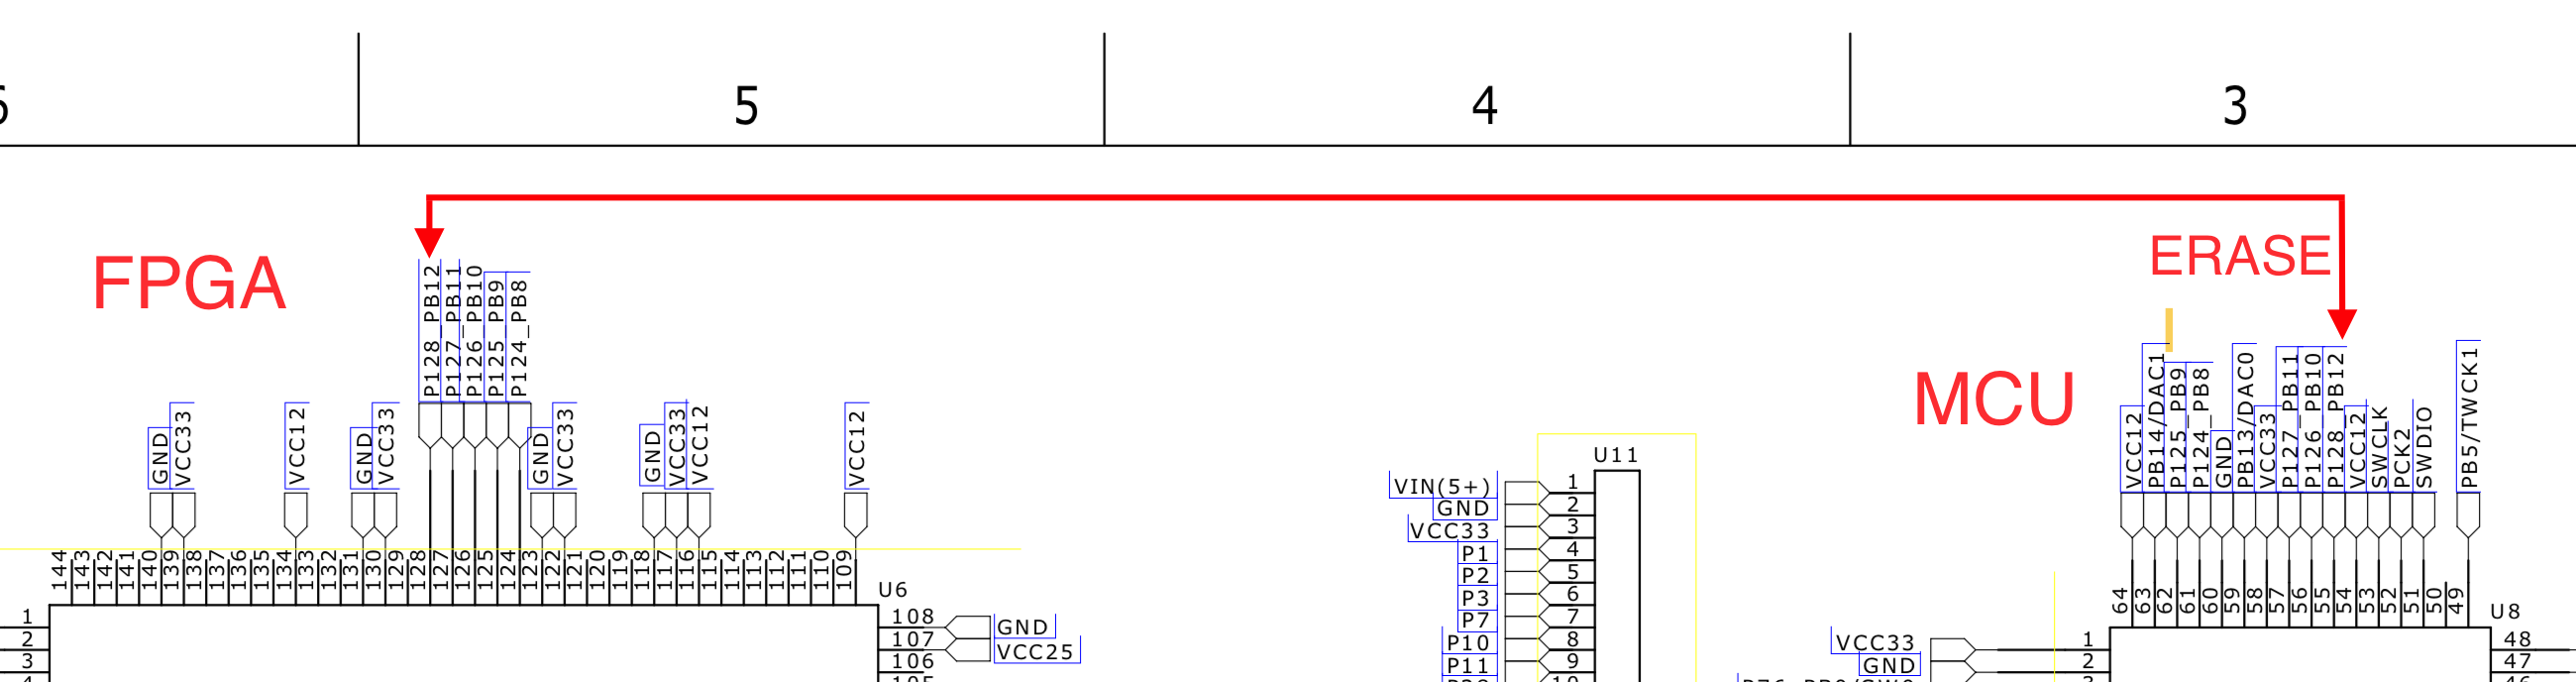
\includegraphics[width=16cm]{erase_error.png}
	\caption{The marked connection ties ERASE on the MCU to pin 128 on the FPGA}
\end{center}

The ERASE pin contains a 100k$\Omega$ pull-down resistor\footnote{SAM4S Series Datasheet p37}.An unconfigured Cyclone IV I/O pin contains a 25k$\Omega$ pull-up resistor \footnote{Cyclone IV Device Handbook p6-3}. This creates a resistor divider circuit as shown below:

\begin{center}
	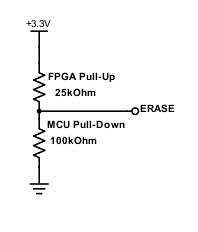
\includegraphics[width=6cm]{resistor_divider.png}
\end{center}

This provides a predicted voltage of 2.64V on the MCU ERASE pin, close to the 2.86V we observed. This is a high logic level which prevented FPGA programming.

\subsubsection{MCU Power Supply}

The MCU requires a 3.3V and 1.2V power supply. It can be powered via one 3.3V supply, and use an internal regulator to generate 1.2V, or it can be powered with an external 3.3V and a 1.2V supply. The dual-regulator design of the current board can introduce startup issues if timing is not correct.

\begin{figure*}
	\begin{center}
	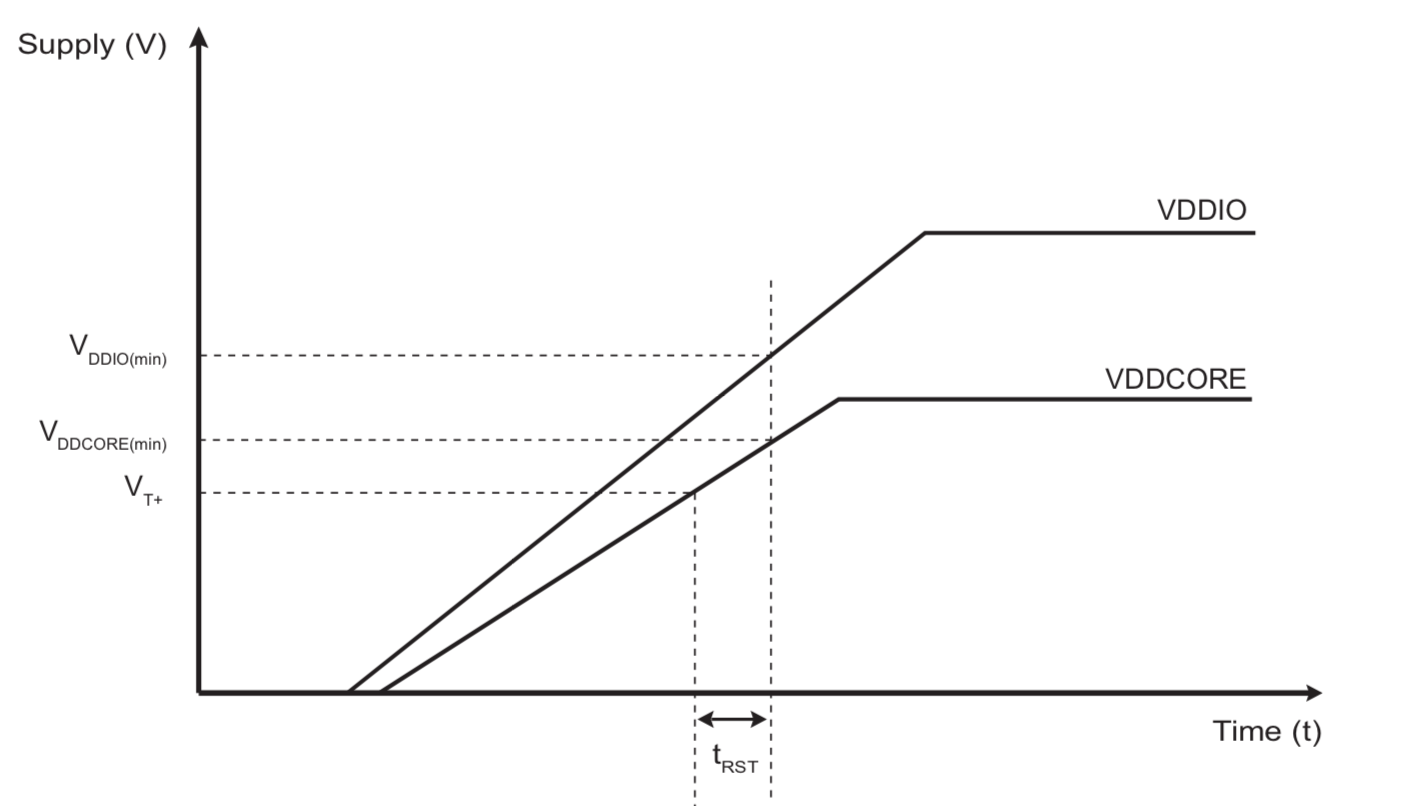
\includegraphics[width=13cm]{power_timing.png}
	\caption{Timing requirements for the 1.2V (VDDCORE) and 3.3V (VDDIO) supplies, taken from the SAM4S Series Datasheet p27}	
	\end{center}
\end{figure*}

We believe that these potential timing errors can cause system instability, as we observed an unresponsive MCU after startup that could only be solved with a full erase and reset.

\subsubsection{JTAG connector pinout}

The MCU JTAG connector was incorrectly wired on the current $\mu$Mudd.

\subsection{Schematic and Layout Changes}

We are currently implementing a set of changes to solve the problems noted above and to improve the PCB. These include:

\begin{enumerate}
	\item Moving ERASE control to the MCU RESET pushbutton. RESET will be accessible through JTAG
	\item Powering the 1.2V MCU VDDCORE with the onboard regulator
	\item Correcting JTAG wiring erros
	\item Replacing 0.1" pitch JTAG connectors with 0.05" pitch SWD connectors. This adds compatibility with J-Link EDU Mini programmers
	\item Adding a separate 40MHz clock to the FPGA. The clock is currently supplied by a MCU I/O pin
\end{enumerate}

\newpage
\section{Deliverable Status: Reworking Lab 6 and EasyPIO.h}

\subsection{Reworking Lab 6}
The proposed Lab 6 architecture is shown in detail below:

\begin{center}
	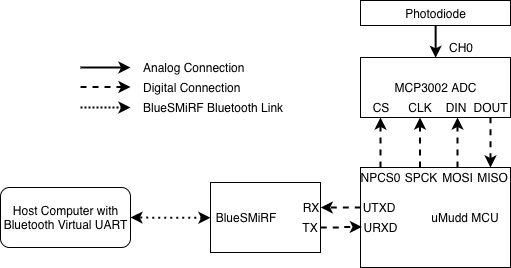
\includegraphics[width=14cm]{blockdiagram.png}
\end{center}

To maintain a low lab cost we exchanged one BlueSMiRF and the serial display for a computer with an integrated bluetooth module. We added a MCP3002 ADC to retain the datasheet interpretation component of the lab.

We have successfully demonstrated bluetooth communication between two computers, using a Bus Pirate as a USB to UART converter. We have also successfully demonstrated voltage measurement with the MCP3002 through a SAM3S/SAM4S SPI peripheral.

The remaining tasks in the rework of Lab 6 are testing our UART peripheral implementation on the SAM3S/SAM4S, and writing an updated version of the lab manual.

\subsection{Targeting EasyPIO.h for the SAM4S}

We aim to create an I/O header file, EasySamIO.h, which provides Arduino-style access to the GPIO, timer, UART, and SPI peripherals on the SAM4S. In the style of EasyPIO.h, we provide only the configuration and functionality necessary to complete labs. We aim to provide adequate inline documentation for students to add functionality as necessary. This documentation includes functional descriptions of memory access, references to the lab manual, and brief descriptions of other peripheral features.

We have completed implementation of the GPIO, timer, and SPI peripherals, and are currently testing our UART implementation.

We believe a thorough and well-documented EasySamIO.h will be more valuable than tests of pre-existing labs as discussed in our project proposal.

\clearpage
\section{Appendix 1: Schematics and Layout}
\clearpage
\section{Appendix 2: C Code}
\subsection{EasySamIO.h}
\subsection{MCP3002 Voltage Measurement}
\subsection{BlueSMiRF UART Communication}
	
\end{document}